\documentclass{bredelebeamer}

\begin{document}

\title[INFO-F-412 - Traffic Light Control]{\textbf{Traffic Light Control} \\INFO-F-412 -- Formal Verification} % The short title appears at the bottom of every slide, the full title is only on the title page

\author[]{Jamal \textsc{Ben Azouze}, Marien \textsc{Bourguignon}, Nicolas \textsc{De Groote}, \\Simon \textsc{Picard}, Arnaud \textsc{Rosette}, Gabriel \textsc{Ekanga}}
\institute[ULB] % Your institution as it will appear on the bottom of every slide, may be shorthand to save space
{
Université Libre de Burxelles \\ % Your institution for the title page
\medskip
\textit{Département d'Informatique} % Your email address
}
\date{4 Juin 2015} % Date, can be changed to a custom date

\begin{frame}
\titlepage % Print the title page as the first slide
\end{frame}

\begin{frame}{Sommaire}
\tableofcontents % Throughout your presentation, if you choose to use \section{} and \subsection{} commands, these will automatically be printed on this slide as an overview of your presentation
\end{frame}

\section{Introduction}
\begin{frame}{First idea}
\centering
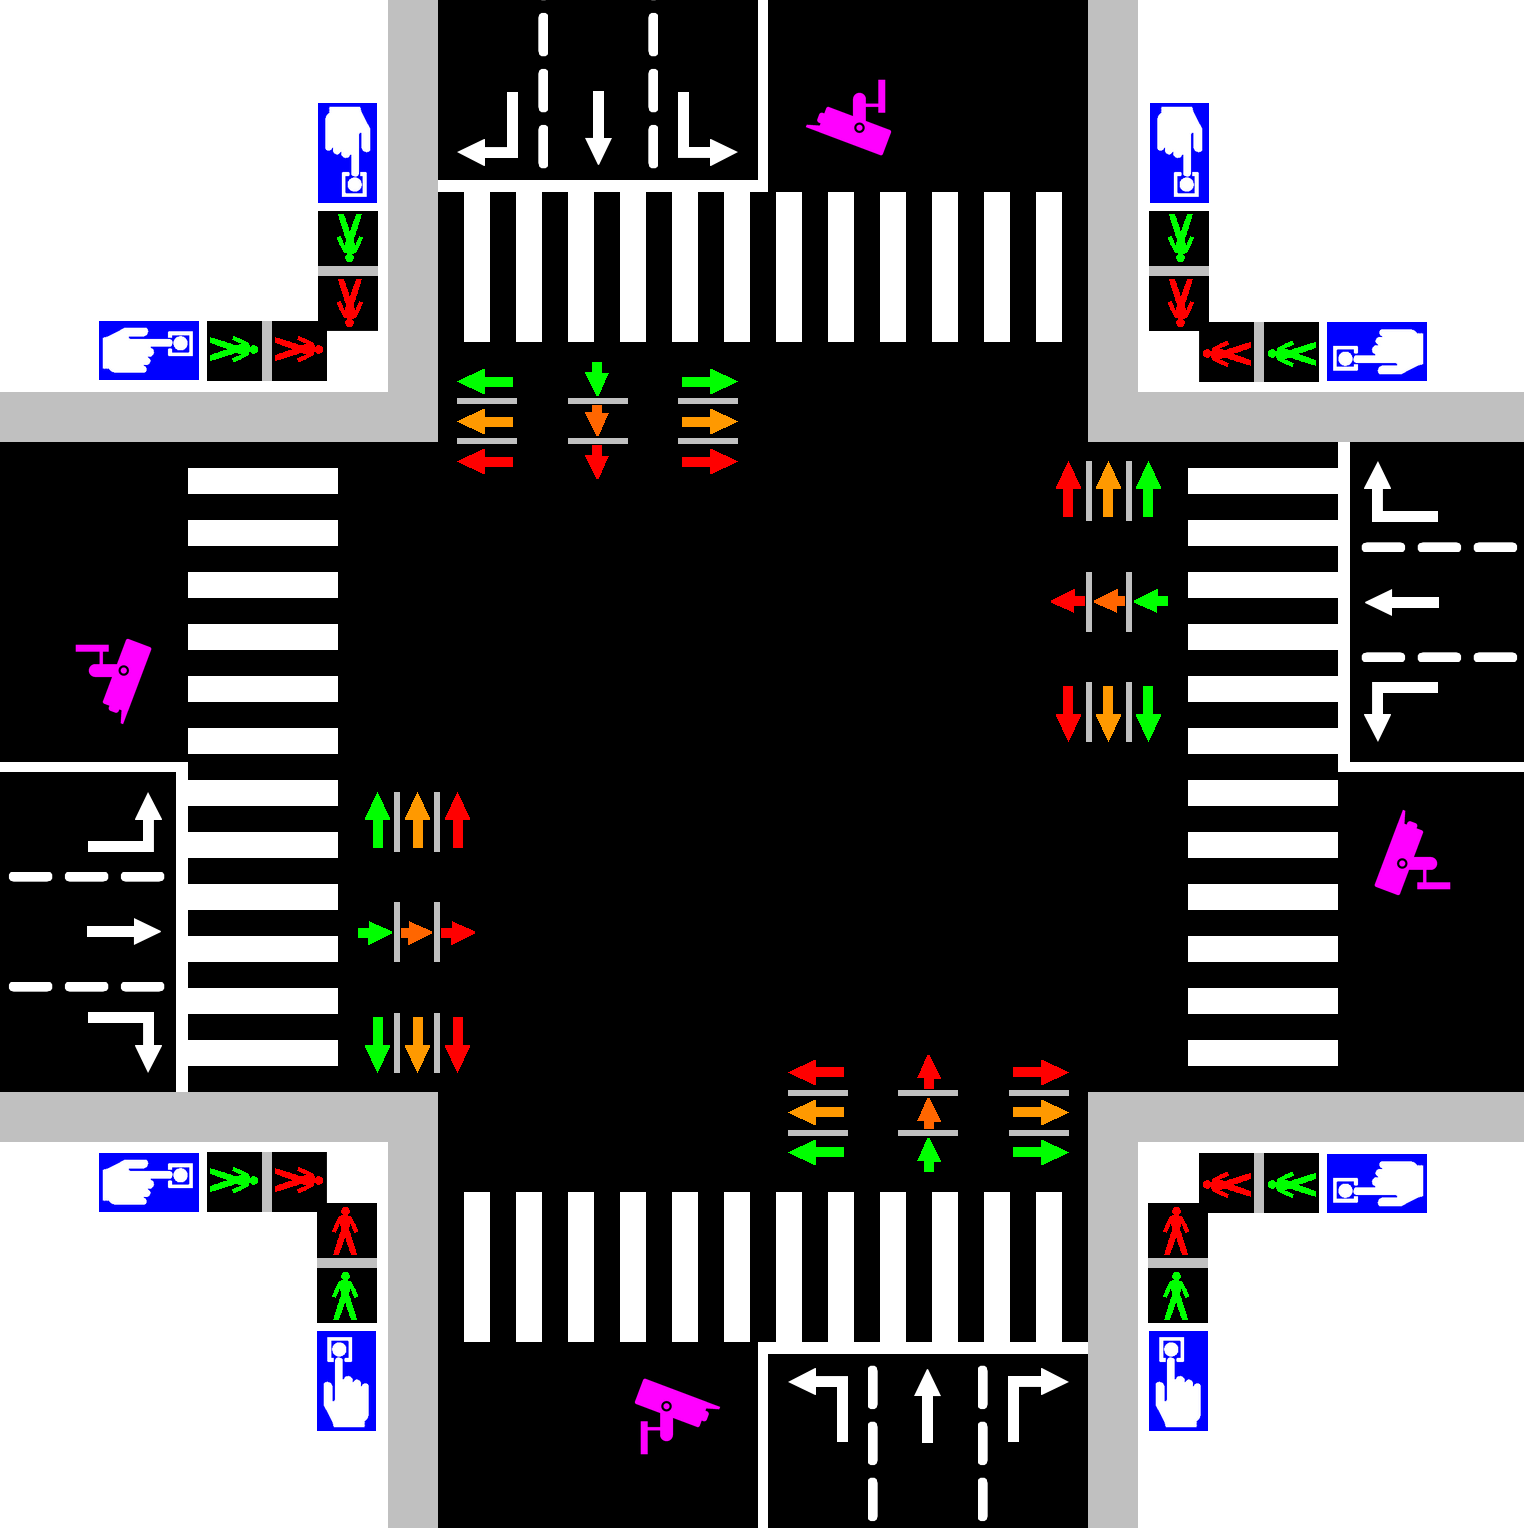
\includegraphics[scale=0.15]{images/idea_draft.png}
\end{frame}
\begin{frame}{Refined idea}
\centering
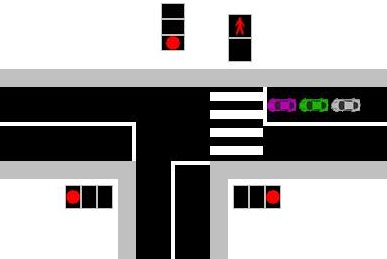
\includegraphics[scale=0.8]{images/final_idea.png}
\end{frame}

\begin{frame}{Assumptions}
\begin{itemize}
\item The traffic lights do not have orange lights -> cars stop instantaneously
\item Every entity respect the highway code 
\item At any time a car can arrive and join a queue of cars
\item At any time a pedestrian can push the button to cross the street
\item A pedestrian will always cross the street in less than a fixed time
\item A car will always cross the crossroads in less than a fixed time
\end{itemize}
\end{frame}

%Est-ce-qu'on fait une slide sur le lien avec embedded system?

%\begin{frame}{Joint project with Embedded System course}

%\end{frame}


\begin{frame}{Benefits of formal verification}
 \begin{itemize}
\item Lives are at stake -> Critical system
\item Impossible to test manually every combination -> Model checking
\end{itemize}
\centering
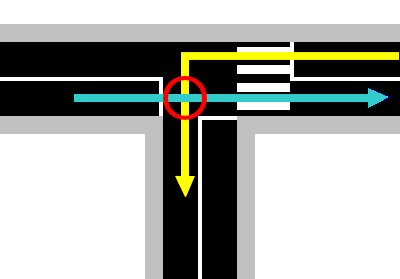
\includegraphics[scale=0.4]{images/exempleCollision.png}
\end{frame}


\section{Uppaal}
\begin{frame}{Uppaal}
\end{frame}

\section{Modeling}

\subsection{Goal}

\begin{frame}{Goal}


\begin{itemize}

\item Important part of the project

\item Expresses the real world thanks to automatons

\\* $\longrightarrow$ will allow to verify the properties

\item Compromises to make between :

\\* - a model with a lot of details which is close to the reality but might be too complex to understand and verify

\\* - a more simple model that would not reflect the reality precisely

\item Importance of identification of the actors

\item Here, we have 3 actors

\\* - Traffic lights

\\* - Pedestrians

\\* - Cars

\end{itemize}


\end{frame}


\subsection{Actors (1) : Traffic lights}

\begin{frame}{Actors (1) : Traffic lights }


\textbf{1) Traffic lights : }


\begin{itemize}

\item They are the main actors in this project

\item They give the authorization to cars and pedestrians to cross the roads at given instants

\item Their role is to schedule the events

\item We assume only that they have only two possible stats (green and red)

\\* $\longrightarrow$ reduces the complexity of the system

\item Orange state is useless

\end{itemize}


\end{frame}


\subsection{Actors (2) : Pedestrians }

\begin{frame}{Actors (2) : Pedestrians }


\textbf{2) Pedestrians : }


\begin{itemize}

\item They come to a traffic light

\item They can push a button

\item wait that the corresponding traffic light passes from red to green in order to cross the road

\item When the traffic light is green, they have a fixed time to cross the road

\end{itemize}


\end{frame}


\subsection{Actors (3) : Cars }

\begin{frame}{Actors (3) : Cars }


\textbf{3) Cars : }


\begin{itemize}

\item They come to a traffic light

\item They wait until they are allowed to enter the crossroad

\item There are several scenarios for them

\item When their traffic light is green, each car can follow different directions

\item We assume that the cars respect the highway code

\end{itemize}


\end{frame}


\subsection{Timed automatons}

\begin{frame}{Timed automatons}


\textbf{Timed automatons : }

\begin{itemize}

\item Used to formally model the system

\item Some of them are part of the environment, the others are part of the controller

\end{itemize}


\textbf{Environment : }

\begin{itemize}

\item Composed of automatons which are not controllable by the system

\item The pedestrians and the cars are unpredictable and uncontrollable

\\* $\longrightarrow$ they belong to the environment

\item Here we have :

\\* - three generators for the cars (one per direction)

\\* - one generator for the pedestrians

\end{itemize}


\end{frame}


\subsection{Automatons of the environment (1) : Pedestrian generator (1/2) }

\begin{frame}{Automatons of the environment (1) : Pedestrian generator (1/2)}


\textbf{Pedestrian generator : }

\newline

\newline


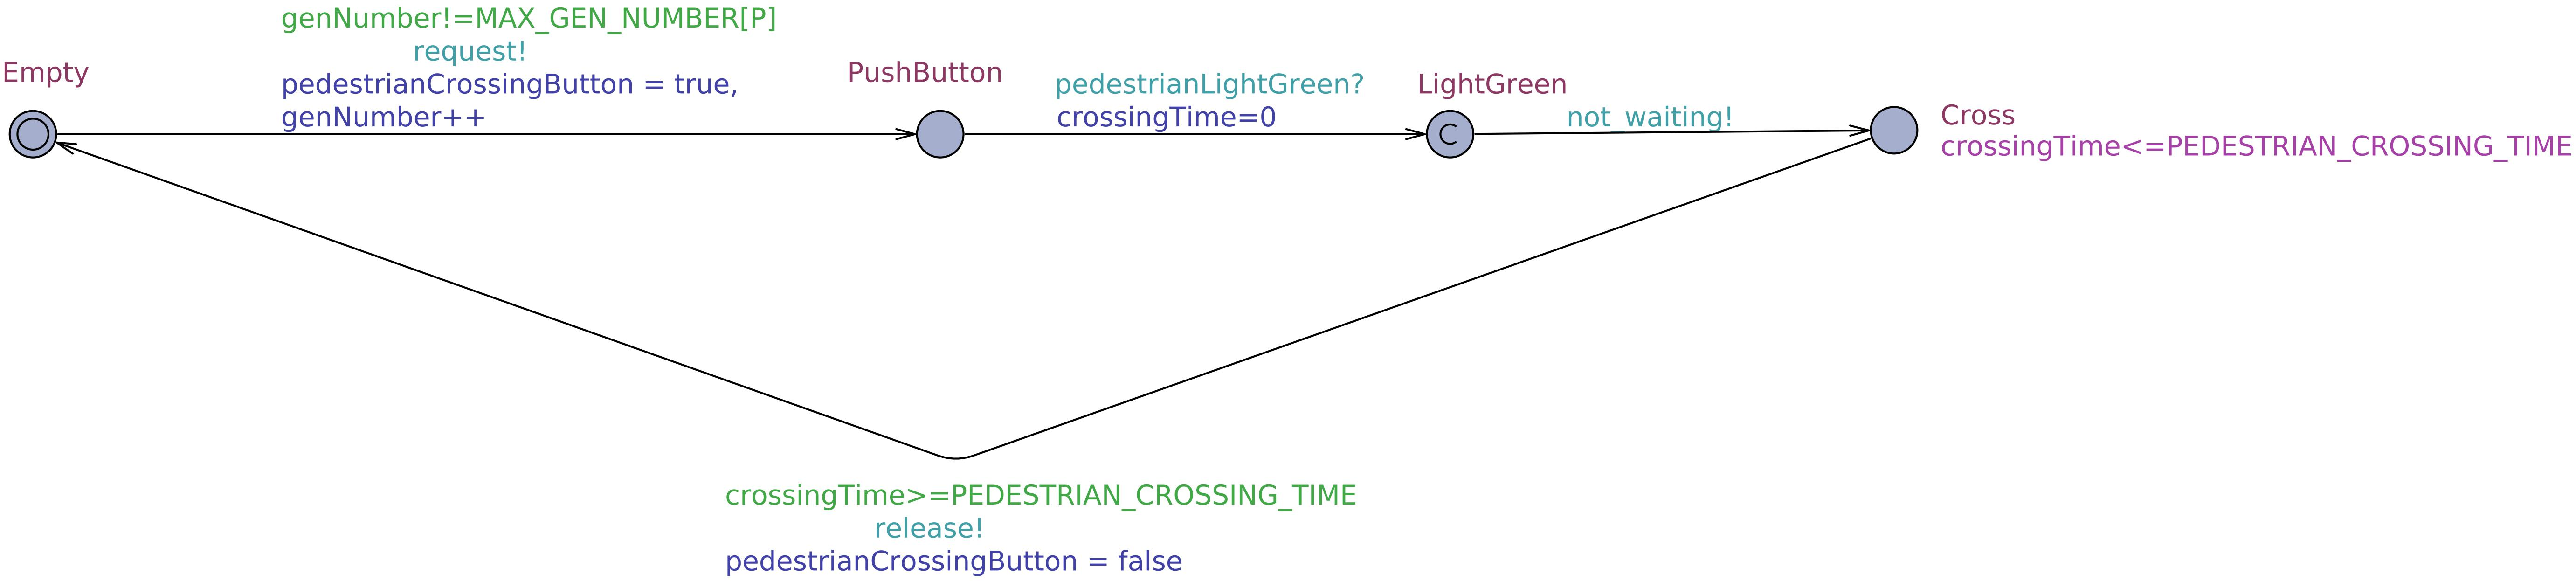
\includegraphics[scale=0.20]{images/imagePedestrianGenerator.jpg}



\end{frame}


\subsection{Automatons of the environment (1) : Pedestrian generator (2/2)}

\begin{frame}{Automatons of the environment (1) : Pedestrian generator (2/2)}


\textbf{Description : }


\begin{itemize}

\item Empty state : initial state, no pedestrian requesting to cross the crosswalk

\item PushButton state : once a pedestrian pushes on the button, stay in this state until the traffic light turns to green

\item LightGreen state : when the light turns to green, the pedestrians cross the road during an undetermined time which is less than a fixed time

\item Cross state : stay in this state during exactly a time equals to the fixed crossing time of the pedestrians before returning the initial state

\end{itemize}


\textbf{Remarks : }


\begin{itemize}

\item In the PushButton state, it cannot receive other requests from other pedestrians because we consider pedestrians as a group of pedestrians and they cross the road in the same time unlike cars

\item There is only one pedestrians generator for the two sides of the crosswalk because the color of the traffic light is the same in the two directions

\item The generator can only generate a fixed number of pedestrian request to reduce the number of the states for the model checking

\end{itemize}


\end{frame}


\subsection{Automatons of the environment (2) : Car generator (1/2)}

\begin{frame}{Automatons of the environment (2) : Car generator (1/2)}


\textbf{Car generator : }

\newline

\newline


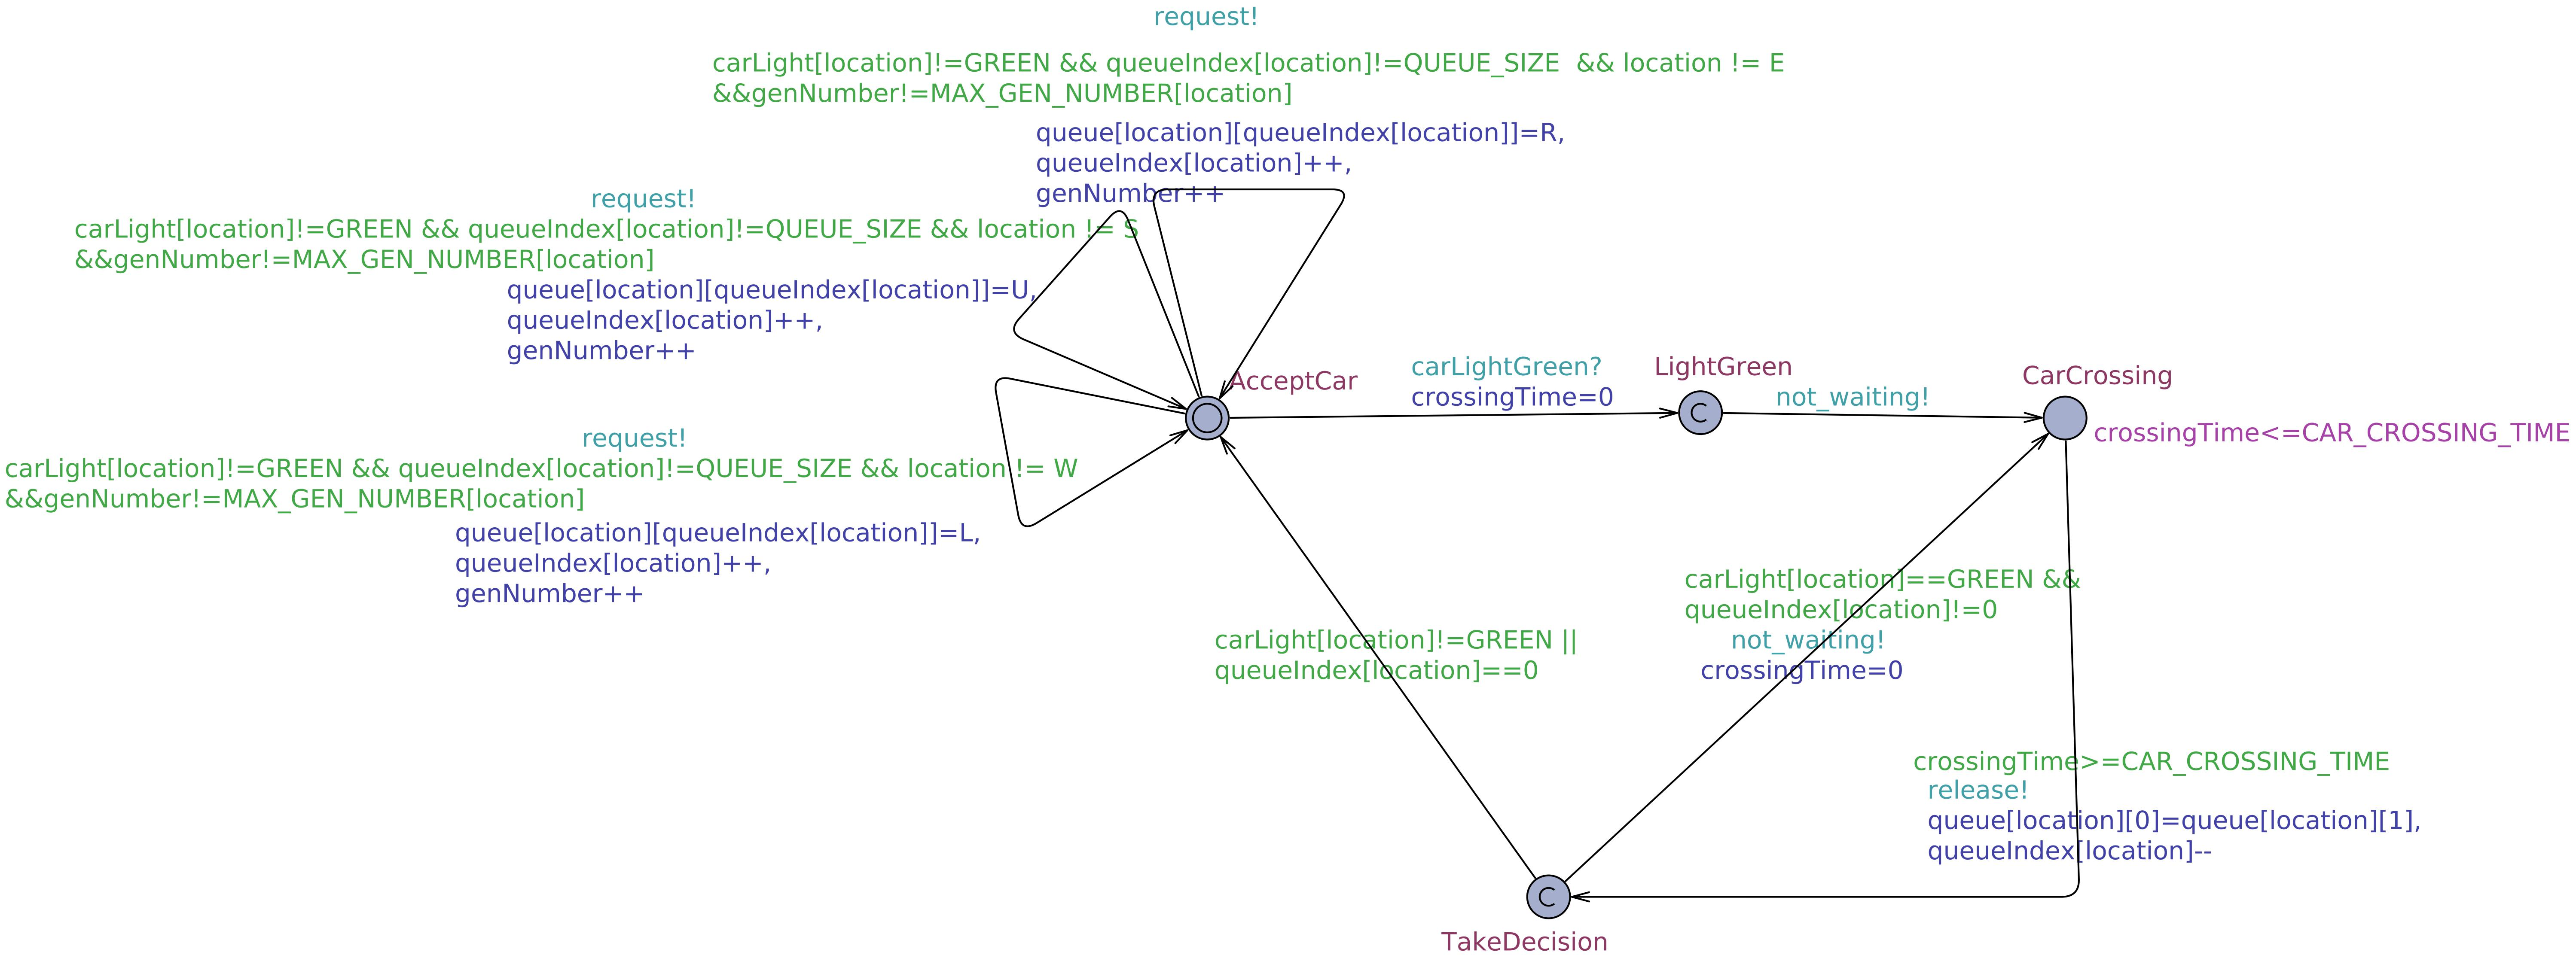
\includegraphics[scale=0.20]{images/imageCarGenerator.jpg}



\end{frame}


\subsection{Automatons of the environment (2) : Car generator (2/2)}

\begin{frame}{Automatons of the environment (2) : Car generator (2/2)}



\textbf{Description : }


\begin{itemize}

\item AcceptCar state: initial state, no cars waiting to cross the crossroad, a car can arrive at any moment if the queue is not full.

\item LightGreen state : once the light becomes green, the first can enter the crossroad

\item CarCrossing state : the cars in the queue continue to cross one by one until the light changes

\item TakeDecision state : returns to the initial state if the light changed to red or the queue is empty, continue to cross if the light is still green and the queue is not empty

\end{itemize}


\textbf{Remarks : }


\begin{itemize}

\item There is three car generators, one for each road

\item Each car generator has a queue storing cars waiting to cross the crossroad, because it has to distinguish each car waiting; unlike the pedestrian generator, the cars do not cross together at the same time

\item the size of the queue equals to two because the time to check properties is too important with more than two locations in the queue and the model is too simple with less locations

\end{itemize}


\end{frame}

\subsection{Controller}
\begin{frame}{Controller}

\end{frame}

\section{Model checking}
\subsection{Liveness properties}
\begin{frame}[fragile]{Liveness properties}

\begin{block}{1. A pedestrian will never wait indefinitely to cross the road}
\begin{verbatim}
p --> q = A[] (p imply A<> q)

PedestrianGeneratorEast.PushButton --> PedestrianGeneratorEast.Cross
\end{verbatim}
\end{block}

\begin{block}{2. A car will never wait indefinitely to enter the crossroad}
\begin{verbatim}
(CarGeneratorEast.AcceptCar&&queueIndex[E]!=0) -->
        CarGeneratorEast.CarCrossing
(CarGeneratorSouth.AcceptCar&&queueIndex[S]!=0) -->
        CarGeneratorSouth.CarCrossing
(CarGeneratorWest.AcceptCar&&queueIndex[W]!=0) -->
        CarGeneratorWest.CarCrossing
\end{verbatim}
\end{block}

\begin{block}{3.No deadlock}
\begin{verbatim}
A[] not deadlock
\end{verbatim}
\end{block}

\end{frame}

\subsection{Safety properties}
\begin{frame}[fragile]{Safety properties}
\begin{block}{1. The pedestrian light will never be green at a wrong time}
\begin{verbatim}
A[] not
(pedestrianLight == GREEN &&
    (carLight[E] == GREEN ||
        (carLight[W] == GREEN && queue[W][0] == U) ||
        (carLight[S] == GREEN && queue[S][0] == R)
    )
)
\end{verbatim}
\end{block}

\begin{block}{2. No pedestrian will be hit by a car}
\begin{verbatim}
A[] not
(PedestrianGeneratorEast.Cross &&
    (CarGeneratorEast.CarCrossing ||
        CarGeneratorWest.CarCrossing && queue[W][0] == U ||
        CarGeneratorSouth.CarCrossing && queue[S][0] == R
    )
)
\end{verbatim}
\end{block}
\end{frame}

\begin{frame}[fragile]{Safety properties}
\centering
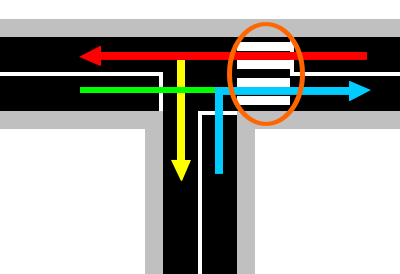
\includegraphics[scale=0.8]{images/pietonCollision.png}

\end{frame}


\begin{frame}[fragile]{Safety properties}

\begin{block}{3. Cars should never collide}
\begin{verbatim}
A[] not (
(
    CarGeneratorWest.CarCrossing && queue[W][0] == U && 
    ((
        CarGeneratorEast.CarCrossing && queue[E][0] == L
    ) || (
        CarGeneratorSouth.CarCrossing && 
        ( queue[S][0] == L || queue[S][0] == R )
    ))
) || (
    CarGeneratorWest.CarCrossing && queue[W][0] == R 
    && CarGeneratorEast.CarCrossing && queue[E][0] == L
))
\end{verbatim}

Same idea for the two other orientations.
\end{block}

\end{frame}
\begin{frame}[fragile]{Safety properties}
\centering
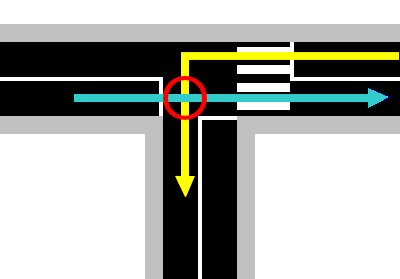
\includegraphics[scale=0.8]{images/exempleCollision.png}

\end{frame}

\begin{frame}[fragile]{Safety properties}
\begin{block}{4. No combination of light allowing car collision}
\begin{verbatim}
A[] not 
(
    (carLight[E] == GREEN && queue[E][0] == L &&
        (
            (carLight[S] == GREEN && queue[S][0] == L) ||
            (carLight[W] == GREEN &&
                (queue[W][0] == U || queue[W][0] == R)
            )
        )
    ) || 
    (carLight[E] == GREEN && queue[E][0] == U &&
    carLight[S] == GREEN && queue[S][0] == L)
)
\end{verbatim}

Same idea for the two other orientations.
\end{block}
\end{frame}


\section{Conclusion}
\begin{frame}{Conclusion}

\begin{block}{Model checking}
Provide tools for verifying system correctness.
\begin{itemize}
\item For a given system and a set of properties (conditions) on this system
\item Determines whether the system satisfies these properties.
\item If not OK, gives a counter-example (optional)
\end{itemize}
\end{block}

\begin{block}{Steps}
\begin{itemize}
\item Catch the real world specifications
\item Determine sets of properties (good, bad, etc.)
\item Model the system using automatons
\item Express the target properties using logic formulas  

\end{itemize}

\end{block}

\end{frame}
\end{document}